%! TeX program = lualatex
\documentclass[main]{subfiles}

\begin{document}

\title[AutoML: BO]{Important Surrogate Models}
\subtitle{Gaussian Processes}
\author[Bernd Bischl]{Bernd Bischl}
\date{}
\titlebackground*{images/AutoML_HPO_2_2}
\maketitle


\begin{frame}{Surrogate Models}
    Desiderata:
    \begin{itemize}
        \item Regression model (there are also classification approaches)
        \item Non-linear local model
        \item Accurate predictions (especially for small sample sizes)
        \item Often: uncertainty estimates
        \item Robust, works often well without human modeler intervention
    \end{itemize}
    Depending on the application:
    \begin{itemize}
        \item Can handle different types of inputs (numerical and categorical)
        \item Can handle dependencies (i.e.\ hierarchical input)
    \end{itemize}
\end{frame}


\begin{frame}{Gaussian Process}
    \small
    Posterior predictive distribution for test point $\conf \in \pcs$ under zero mean:
    $$Y(\conf) \mid \conf, \Dt \sim \normal\left(\surro(\conf), \sh^2(\conf)\right)$$
    with
    $$\surro(\conf) = k(\conf)^\top \bm{K}^{-1} \yv, \quad \sh^2(\conf) = k(\conf, \conf) - k(\conf)^\top \bm{K}^{-1} k(\conf)$$
    \begin{center}
        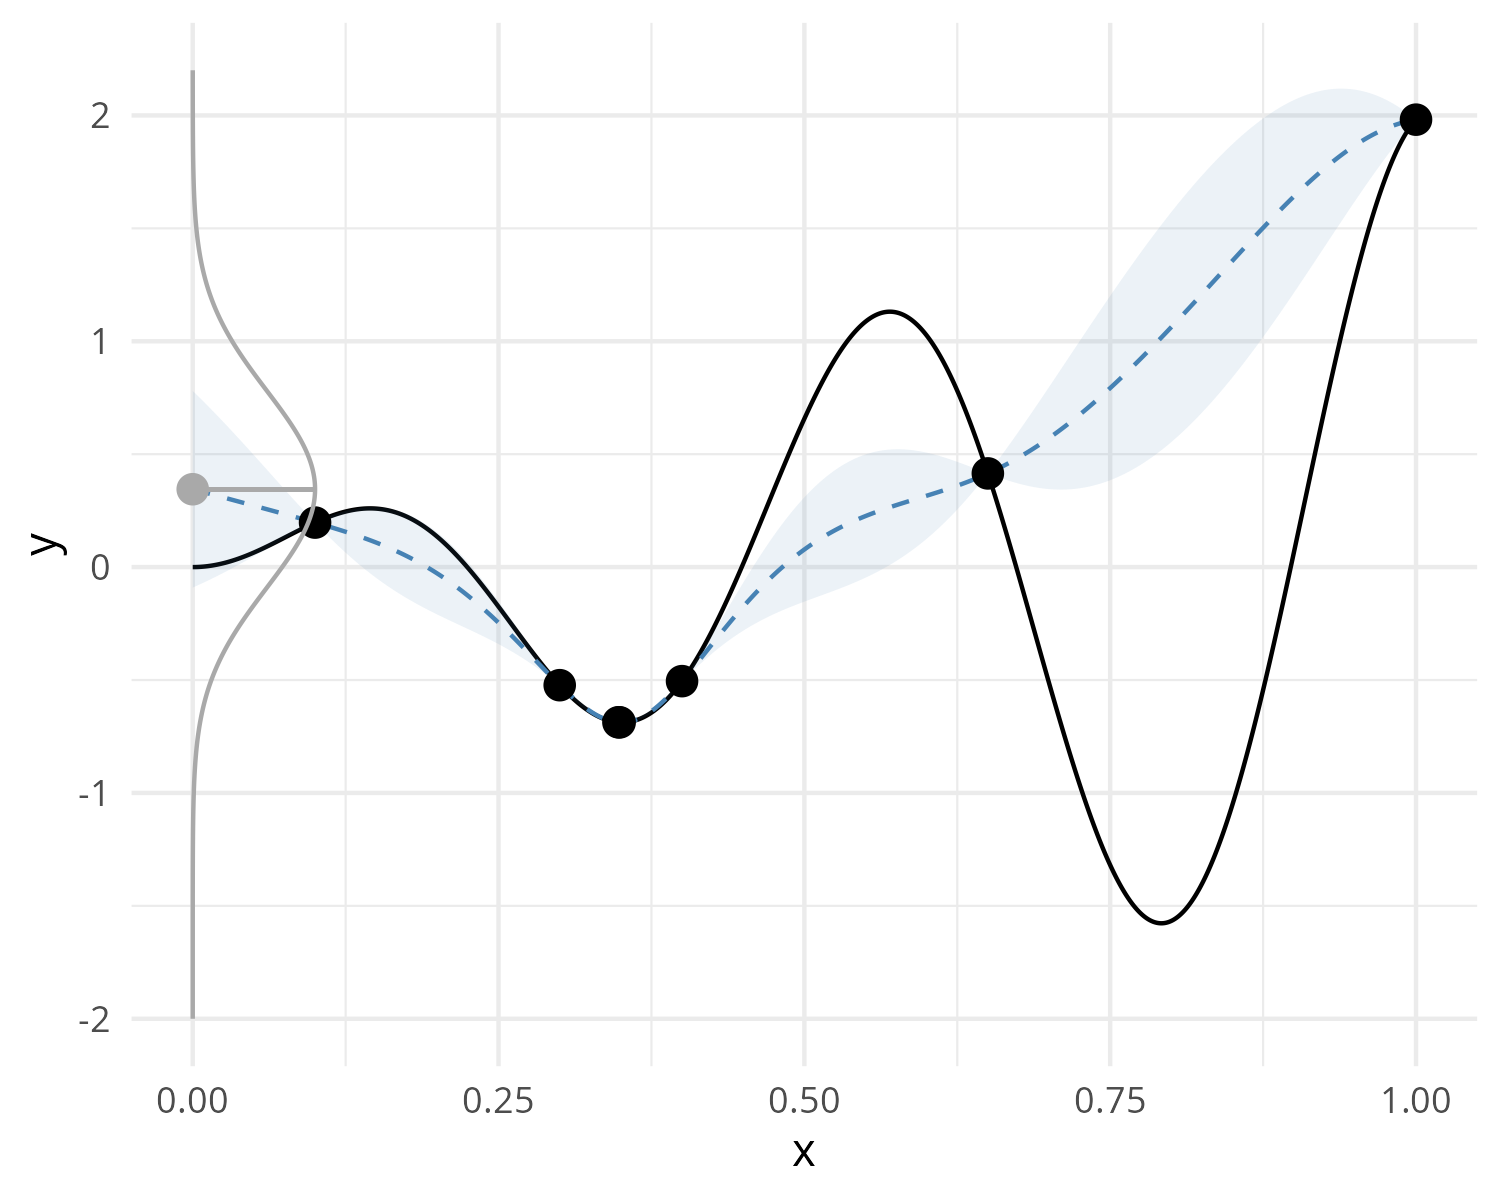
\includegraphics[width=.4\textwidth]{images/bayesian_loop_sm_normal.png}
    \end{center}
    \footnotesize Note: $\conf$ here denotes the test input. $k(\conf) := (k(\conf, \confI{1}), \ldots, k(\conf, \confI{t}))^\top$, $\yv := (\ysi[1], \ldots, \ysi[t])^\top$. Kernel/Gram matrix $\bm{K} := (k(\confI{i}, \confI{j}))_{i,j}$ for $i, j \in \{1, \ldots, t\}$.
\end{frame}


\begin{frame}{Gaussian Process}
    \small
    Example kernel functions:
    \begin{itemize}
        \item Radial basis function kernel (aka Gauss kernel):
        $$k(\conf, \conf') = \exp\!\left(-\frac{d(\conf, \conf')^2}{2 l^2}\right)$$
        \begin{itemize}
            \item $l$ length scale; $d(\cdot, \cdot)$ Euclidean distance
            \item Infinitely differentiable -- very ``smooth''
        \end{itemize}
        \item Matérn kernels:
        $$k(\conf, \conf') = \frac{1}{\Gamma(\nu)\, 2^{\nu-1}}\left(\frac{\sqrt{2\nu}}{l} d(\conf, \conf')\right)^\nu K_\nu\!\left(\frac{\sqrt{2\nu}}{l} d(\conf, \conf')\right)$$
        \begin{itemize}
            \item $l$ length scale; $K_\nu(\cdot)$ modified Bessel function; $\Gamma(\cdot)$ Gamma function
            \item For $\nu = 3/2$ once differentiable, for $\nu = 5/2$ twice differentiable
            \item Popular choice as a kernel function when using a GP as SM
        \end{itemize}
    \end{itemize}
\end{frame}


\begin{frame}{Gaussian Process}
    \textbf{Pros:}
    \begin{itemize}
        \item Smooth, local, powerful estimator, also for small data
        \item GPs yield well-calibrated uncertainty estimates
        \item The posterior predictive distribution under a GP is normal
    \end{itemize}
    \textbf{Cons:}
    \begin{itemize}
        \item Vanilla GPs scale cubically in the number of data points
        \item Can natively only handle numeric features; mixed inputs / dependencies require special kernels
        \item Not that robust; numerical problems can occur
        \item Can be sensitive to the choice of kernel and hyperparameters
    \end{itemize}
\end{frame}

\begin{frame}{Summary}
\begin{enumerate}
    \item A good BO surrogate provides accurate, uncertainty-aware predictions and handles mixed input types if needed
    \item Gaussian processes are the default choice: well-calibrated uncertainty, but limited scalability and robustness
    \item Random forests scale better and handle mixed/hierarchical spaces, at the cost of weaker uncertainty estimates
\end{enumerate}
\end{frame}

\end{document}
